\documentclass{beamer}
\usepackage{subcaption}
\usepackage{float}
\usepackage{setspace}
\usepackage{wrapfig}
\usepackage{caption}
\usepackage{mwe,tikz}\usepackage[percent]{overpic}
\captionsetup[figure]{labelformat=empty}
\usepackage{multirow}
\usepackage{array}
\usepackage{longtable}
\usepackage{pdfpcnotes}
\newcolumntype{L}[1]{>{\raggedright\let\newline\\\arraybackslash\hspace{0pt}}m{#1}}
\newcolumntype{C}[1]{>{\centering\let\newline\\\arraybackslash\hspace{0pt}}m{#1}}
\newcolumntype{R}[1]{>{\raggedleft\let\newline\\\arraybackslash\hspace{0pt}}m{#1}}
\usetheme[pageofpages=of,% String used between the current page and the
                         % total page count.
          bullet=circle,% Use circles instead of squares for bullets.
          titleline=true,% Show a line below the frame title.
          alternativetitlepage=true,% Use the fancy title page.
          titlepagelogo=logo-polito,% Logo for the first page.
          watermark=watermark-polito,% Watermark used in every page.
          watermarkheight=100px,% Height of the watermark.
          watermarkheightmult=4,% The watermark image is 4 times bigger
                                % than watermarkheight.
          ]{Theme}
\usepackage{lmodern}
\author{\small By\\Bharat Bhushan (153100048)}
\title{{{Thermoelastic fracture problems using Extended Finite\vspace{.3cm} Element Method}}}
\institute{\small Under the guidance of\\Prof. Salil S. Kulkarni\\ \vspace{5pt}Department of Mechanical Engineering, IIT Bombay}
\date{\vspace{-5pt}\today}
\begin{document}
%%%%%%%%%%%%%%%%%%%%%%%%%%%%%%%%%%%%%%%%%%%%%%%%%%%%%%%%%%%%%%%%%%%%5
%%%% TITLE PAGE %%%%%%%%%%%%%%%%%%%%%%%%%%%%%%%%%%%%%%%%%%%%%%%%%%%%
%%%%%%%%%%%%%%%%%%%%%%%%%%%%%%%%%%%%%%%%%%%%%%%%%%%%%%%%%%%%%%%%%%%%%
\begin{frame}[t,plain]
\titlepage
\end{frame}
%%%%%%%%%%%%%%%%%%%%%%%%%%%%%%%%%%%%%%%%%%%%%%%%%%%%%%%%%%%%%%%%%%%%%%
%%%% content %%%%%%%%%%%%%%%%%%%%%%%%%%%%%%%%%%%%%%%%%%%%%%%%%%%%%%%
%%%%%%%%%%%%%%%%%%%%%%%%%%%%%%%%%%%%%%%%%%%%%%%%%%%%%%%%%%%%%%%%%%%%

%%%%%%%%%%%%%%%%%%%%%%%%%%%%%%%%%%%%%%%%%%%%%%%%%%%%%%%%%%%%%%%%%
\begin{frame}[t,fragile]{Outline}
    \begin{itemize}
        \item Introduction 
        \item Motivation 
        \item Literature Survey 
        \item Work done 
        \item Problem definition 
        \item Conclusion 
    \end{itemize}
\end{frame}
%%%%%%%%%%%%%%%%%%%%%%%%%%%%%%%%%%%%%%%%%%%%%%%%%%%%%%%%%%%%%%%%%
\begin{frame}[t,fragile]{Introduction: Thermo-elastic Fracture Mechanics}
    \vspace{-.3cm}
    \footnotesize
    \begin{itemize}
\onslide<1->        \item Thermo-elastic Fracture mechanics is a field of mechanics where we study the propagation of crack in materials in presence of temperature field.
 \onslide<2->       \item Due to heat transfer, temperature field is set up in the material which induces thermal stresses in the body. 
     \onslide<3-> \item These stresses becomes very large around a discontinuity i.e crack tip. If temperature variation is sufficiently large, it can lead to failure.
   \onslide<4->     \item Applications: Nuclear power plants, cylinder-nozzle
 intersection in pressure vessels, aerodynamic heating of high-speed aircraft, ultra fast pulse lasers etc.
   \end{itemize}
   \vspace{-.5cm}
\begin{figure}[H]
    \hspace{.7cm}
      \begin{subfigure}{0.45\textwidth}
    \centering
 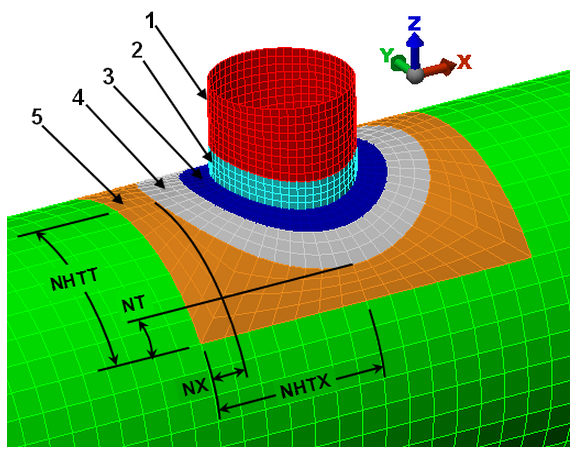
\includegraphics[scale=.1]{cyl.png}
 \caption{\tiny{The cylinder-nozzle intersection. (www.knowledge.autodesk.com)}}
 \label{cyl}
 \end{subfigure}
\begin{subfigure}{0.45\textwidth}
    \centering
 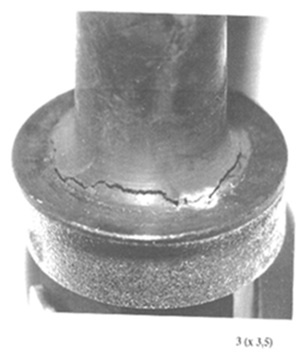
\includegraphics[scale=.1]{fail.jpg}
 \caption{\tiny{Cracked head of baffle bolt of Belgian Nuclear Reactor.(www.miningawareness.wordpress.com)}}
 \label{fail}
 \end{subfigure}
 \end{figure}
 \vspace{-.3cm}
   \tiny
   \hspace{15pt}
   \textbf{source}: Tian, X., Shen. (2006). A direct finite element method study of generalized thermoelastic problems. \\
   \vspace{-7pt}
   \hspace{15pt}
   \emph{International Journal of Solids and Structures}, 43(7), 2050-2063.
\end{frame}
%%%%%%%%%%%%%%%%%%%%%%%%%%%%%%%%%%%%%%%%%%%%%%%%%%%%%%%%%%%%%%%%%o 
\begin{frame}[t,fragile]{Why thermal load on crack is important?}
    \vspace{-.3cm}
    \footnotesize
\begin{itemize}
\onslide<2->    \item Atkinson has solved the Dirichlet problem for Laplace's equation on a pie shaped region as $u(x,y)= r^{\frac{\pi}{\phi}}\sin\alpha\theta,\  r>0,\ 0<\theta<\phi$
        \begin{itemize}
                \footnotesize
    \onslide<3->\item If $0<\phi<\pi$:
        The first partial derivative of u with respect to x and y remains continuous as we approach towards the origin. 
  \onslide<4->  \item If $\pi<\phi<2\pi$:
        The first derivative u with respect to x and y are not continuous as (x,y) approaches the origin. 
      \onslide<5-> \item When $\phi=2\pi$, the problem becomes a crack problem and displacement and derivative of displacement vary as $u \propto r^{\frac{1}{2}}$ and $u'\propto  r^{-\frac{1}{2}}$ respectively. 
  \end{itemize}
 \onslide<6->  \item As thermo-elastic problems are also governed by Laplace's equation, temperature will vary as $r^{\frac{1}{2}}$ and heat fluxes will be unbounded at the crack tip. 
\end{itemize}
  \tiny
  \vspace{10pt}
  \hspace{10pt}
   \textbf{source}: Atkinson, K. E. (1997).
    \emph{The numerical solution of \\
  \hspace{10pt}
    integral equations of the second kind} (Vol. 4). \\
  \hspace{10pt}
    Cambridge university press.
    \onslide<2-> \begin{wrapfigure}{r}{0.4\textwidth}
    \centering
    \vspace{-50pt}
    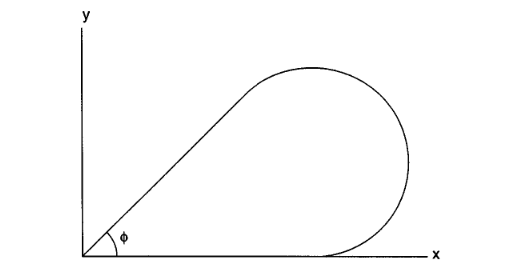
\includegraphics[width=.3\textwidth]{pie.png}
    \caption{\footnotesize Pie-shaped region.}
    \label{pie}
\end{wrapfigure}
 
\end{frame}
%%%%%%%%%%%%%%%%%%%%%%%%%%%%%%%%%%%%%%%%%%%%%%%%%%%%%%%%%%%%%%%%%%%%
\begin{frame}[t,fragile]{Extended Finite Element Method in Thermoelasticity}
    \vspace{-.5cm}
    \small
    \begin{itemize}
       \onslide<2-> \item In FEM we have to use very fine mesh to capture the behaviour of crack.\onslide<3->
\item In X-FEM, we enrich the polynomial approximation to include the effects of singular discontinuous field.
   \onslide<4-> \item Advantages:
    \begin{itemize}
       \onslide<5-> \item Mesh is prepared without considering the existence of discontinuity
        \onslide<6->\item No need of remeshing
     \onslide<7->   \item Accurate solution
    \end{itemize}
\end{itemize}\onslide<3->
\begin{figure}
     \centering
     \vspace{-10pt}
     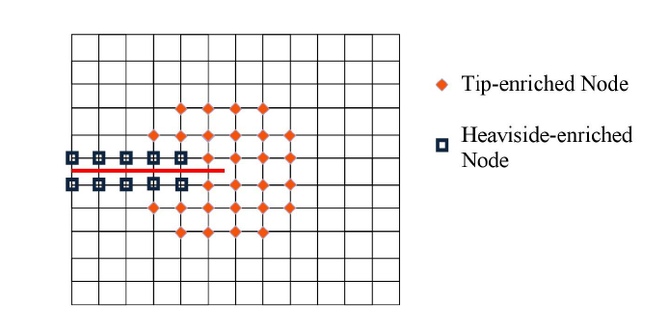
\includegraphics[scale=.3]{enrich.png}
     \vspace{-.4cm}
     \caption{\hspace{-2cm}\footnotesize X-FEM enrichment strategy}
  \end{figure}
\end{frame}
%%%%%%%%%%%%%%%%%%%%%%%%%%%%%%%%%%%%%%%%%%%%%%%%%%%%%%%%%%%%%%%%%%%%%%%%%%%%
%%%%%%%%%%%%%%%%%%%%%%%%%%%%%%%%%%%%%%%%%%%%%%%%%%%%%%%%%%%%%%%%%%%%%%%%%%%%
\begin{frame}[t,fragile]{Two types of enrichment functions in X-FEM}
    \vspace{-.3cm}
     \footnotesize
    \begin{itemize}
 \onslide<2->       \item The nodes which belongs to the elements totally cut by the crack, are enriched by and Heaviside function.
    $$h(x,y)=\begin{cases}1,&       for ~ ~ y\ge 0\\ -1,&       for~ ~ y\le 0\end{cases}$$\onslide<3->
\item The nodes of elements which contains cracktip are enriched by $\gamma$:
     \footnotesize
    \begin{align*}
     u^h&=\sum_i N_i(x)u_i+\sum_{j\in J} N_j(x) h(x)a_j+\sum_{k\in K} N_k(x)\left( \sum_{l=1}^{4}\gamma_l(x)b_{kl} \right) \\
    v^h&=\sum_i N_i(x)v_i+\sum_{j\in J} N_j(x) h(x)c_j+\sum_{k\in K} N_k(x)\left( \sum_{l=1}^{4}\gamma_l(x)d_{kl} \right) \\ 
     where,\ \ \ \gamma&=\left[ \sqrt{r}\cos \left( \frac{\theta}{2} \right), \sqrt{r}\sin\left( \frac{\theta}{2} \right),\sqrt{r}\sin\left( \frac{\theta}{2} \right)\sin(\theta),\sqrt{r}\cos\left( \frac{\theta}{2} \right)\sin(\theta)\right] 
\end{align*}
\end{itemize}
\tiny
\hspace{10pt}
\textbf{Source:}Belytschko, T., \& Black, T. (1999). Elastic crack growth in finite elements with minimal remeshing. \\
\vspace{-7pt}
\hspace{10pt}
\emph{International journal for numerical methods in engineering}, 45(5), 601-620.
\end{frame}
%%%%%%%%%%%%%%%%%%%%%%%%%%%%%%%%%%%%%%%%%%%%%%%%%%%%%%%%%%%%%%%%%%%%%%%%
\begin{frame}[t,fragile]{Which Nodes to Enrich? - Level Set Method}
    \vspace{-.3cm}
    \footnotesize
    \begin{itemize}
      \onslide<2->  \item There are two level-set functions defined as follows:
       \onslide<3->   \begin{itemize}
        \item Normal level set, $\psi(x)=$ the signed distance from the crack surface.
     \onslide<4->   \item Tangent level set, $\phi(x)=$ the signed distance to the plane including the crack front and perpendicular to the crack surface.
        \end{itemize}
  \onslide<5->  \item To decide which enrichment should be used. 
        \begin{itemize}
     \onslide<6->       \item If $\phi < 0 $ and $\psi_{min}\psi_{max}\leq 0$, nodes should be enriched with $h(x)$.
       \onslide<7->     \item If $\phi_{min}\phi_{max}\leq 0$ and $\psi_{min}\psi_{max}\leq 0 $, nodes should be enriched with $\gamma$.
        \end{itemize}
    \end{itemize}
 \onslide<3-> \begin{figure}
                \centering
                \vspace{-15pt}
                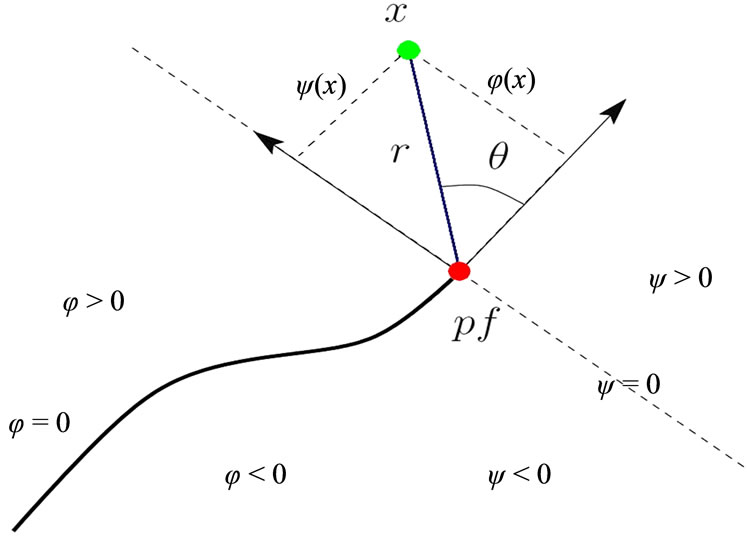
\includegraphics[scale=.15]{levelset.jpg}
                \caption{\tiny Level Set Method}
                \label{4}
            \end{figure}
    \tiny 
    \vspace{-20pt}
  \hspace{10pt}
    \textbf{Source:} Abdelaziz, Y., Bendahane, K., \& Baraka, A. (2011). Extended Finite Element Modeling: Basic Review and\\
  \vspace{-1pt}
  \hspace{10pt}
    Programming. Engineering, 3(07), 713.

\end{frame}
%%%%%%%%%%%%%%%%%%%%%%%%%%%%%%%%%%%%%%%%%%%%%%%%%%%%%%%%%%%%%%%%%%%%%%%%%%%%%%%
\begin{frame}[t,fragile]{Work Done}
    \begin{itemize}
      \onslide<2->  \item Finite Element Formulation of coupled thermoelasticity 
       \onslide<3-> \item Development of a MATLAB program for semi-coupled thermoelastic problems.
   \onslide<4->     \item Patch tests to validate the developed FEM program.
   \onslide<5->     \item Solution of various thermoelastic fracture problems and comparison with the analytical solutions. 
   \onslide<6->     \item Comparison between the results of FEM and X-FEM programs. 
    \end{itemize}
\end{frame}
%%%%%%%%%%%%%%%%%%%%%%%%%%%%%%%%%%%%%%%%%%%%%%%%%%%%%%%%%%%%%%%%%%%
\begin{frame}[t,fragile]{Finite Element Formulation of Thermo-elasticity}
\begin{itemize}\onslide<2->
\item We have formulated the semi-coupled in which we neglected the effect of displacements on temperature field.\onslide<3->
\item In thermoelastic case the total strain is given as: 
\begin{align*}
    \varepsilon_{ij}&=\varepsilon_{ij}^{(M)}+\varepsilon_{ij}^{(T)}
    =\frac{1+\nu}{E}\sigma_{ij}-\frac{\nu}{E}\sigma_{kk}\delta_{ij}+\alpha(T-T_0)\delta_{ij}\nonumber
\end{align*}
\onslide<4->
\item It can be inverted to get following stress-strain relationship:
    \footnotesize
\begin{align*}
    \begin{Bmatrix}
        \sigma_{x}\\ \sigma_{y}\\ \tau_{xy} 
    \end{Bmatrix} =\frac{E}{(1-\nu^2)}
    \begin{bmatrix}
        1 & \nu & 0 \\ \nu & 1 & 0 \\ 0 & 0 & 1-\nu 
    \end{bmatrix}
    \begin{Bmatrix}
        \varepsilon_{x}-\alpha\Delta T \\ \varepsilon_{y}-\alpha \Delta T \\ \varepsilon_{xy} 
    \end{Bmatrix}
\end{align*}
\end{itemize}

\end{frame}
%%%%%%%%%%%%%%%%%%%%%%%%%%%%%%%%%%%%%%%%%%%%%%%%%%%%%%%%%%%%%%%
   \begin{frame}[t,fragile]{Governing Equations of Thermoelasticity}
    \begin{itemize}
       \onslide<2-> \item The governing equations of the thermo-elasticity is derived as: 
            \bgroup
            \footnotesize
            \begin{align*}
    \frac{\partial}{\partial x}\left[c_{11}\frac{\partial u}{\partial x}+c_{12}\frac{\partial v}{\partial y}\right]+&\frac{\partial}{\partial y}\left[c_{66}\left(\frac{\partial u}{\partial y}+\frac{\partial v}{\partial x}\right)\right]-(c_{11}+c_{12})\alpha\frac{\partial T}{\partial x}-f_x   =0 \\
    \frac{\partial}{\partial x}\left[c_{66}\left(\frac{\partial u}{\partial y}+\frac{\partial v}{\partial x}\right)\right]+&\frac{\partial}{\partial y}\left[c_{12}\frac{\partial u}{\partial x}+c_{22}\frac{\partial v}{\partial y}\right]-(c_{11}+c_{12})\alpha\frac{\partial T}{\partial y}-f_y=0\\
    &\ \ \ \ \ \ \ k\left( \frac{\partial^2 T}{\partial x^2}+\frac{\partial^2 T}{\partial y^2} \right)=q
\end{align*}
\egroup
     \onslide<3-> \item We can develop a week form of above equations by approximating u,v and T over a typical finite element $\Omega^e$ as:
          \footnotesize
\begin{align*}
    u(x,y)=\sum_{i=1}^nN_i (x,y)u_i\ \ , 
    v(x,y)=\sum_{i=1}^nN_i (x,y)v_i\ \ ,
    T(x,y)=\sum_{i=1}^nN_i (x,y)T_i
\end{align*}
\end{itemize}
\end{frame}
%%%%%%%%%%%%%%%%%%%%%%%%%%%%%%%%%%%%%%%%%%%%%%%%%%%%%%%%%%%%%%%%%%%%%%
\begin{frame}[t,fragile]{Weak Form Equations of Coupled Thermoelasticity}
    \vspace{-.4cm}
            \scriptsize
      \onslide<2->  \begin{align*}
     -\int_{\Omega}^{}\left[ c_{11}\frac{\partial N_i}{\partial x}\frac{\partial N_j}{\partial x}u_j+c_{12}\frac{\partial N_i}{\partial x}\frac{\partial N_j}{\partial y}v_j\right]dxdy+\int_{\Omega}^{}\left[c_{66}\frac{\partial N_i}{\partial y}\frac{\partial N_j}{\partial y}u_jdxdy+\frac{\partial N_i}{\partial y}\frac{\partial N_j}{\partial x}v_j\right]dxdy\nonumber\\ -\int_{\Omega}^{}\frac{\partial N_i}{\partial x}\beta N_jT_j dxdy +\int_{\Omega}^{}N_if_x
     dxdy+\int_{\Gamma}^{}N_i\vec{t}dx=0\end{align*}
 \onslide<3->\begin{align*}
     -\int_{\Omega}^{}\left[ c_{11}\frac{\partial N_i}{\partial y}\frac{\partial N_j}{\partial y}v_j+c_{12}\frac{\partial N_i}{\partial y}\frac{\partial N_j}{\partial x}u_j\right]dxdy+\int_{\Omega}^{}\left[c_{66}\frac{\partial N_i}{\partial x}\frac{\partial N_j}{\partial x}v_jdxdy+\frac{\partial N_i}{\partial x}\frac{\partial N_j}{\partial y}u_j\right]dxdy\nonumber\\ -\int_{\Omega}^{}\frac{\partial N_i}{\partial y}\beta N_jT_j dxdy+\int_{\Omega}^{}N_if_y dxdy+\int_{\Gamma}^{}N_i\vec{t}dy=0
 \end{align*}
 \onslide<4->\begin{align*}
        k\int_{\Omega}\left( \frac{\partial N_i}{\partial x}\frac{\partial N_j}{\partial x}+\frac{\partial N_i}{\partial y}\frac{\partial N_j}{\partial y} \right)T_jdxdy-\int_{\Omega}^{}N_iN_jqdxdy=\int_{\Gamma}^{}N_i\bar{Q}ds& \end{align*}
\end{frame}
%%%%%%%%%%%%%%%%%%%%%%%%%%%%%%%%%%%%%%%%%%%%%%%%%%%%%%%%%%%%%%%%%%%
\begin{frame}[t,fragile]{Finite Element Model}
    \vspace{-.3cm}
    \footnotesize
    \begin{itemize}
      \onslide<2->  \item Neglecting the body forces, above equations can be written in matrix form as: 
    \begin{align*}
\begin{bmatrix}
    K_{11} & K_{12} \\
    0 & K_{22}
\end{bmatrix}
\begin{Bmatrix}
    U^e\\ T^e
\end{Bmatrix}=
\begin{Bmatrix}
    F\\ Q
\end{Bmatrix}
\end{align*}\onslide<3->
Where,
\vspace{-.2cm}
    \scriptsize 
\begin{align*}
    [K_{11}^e]=\int_{\Omega}[B]^T[C][B]dxdy\ \
    [K_{12}^e]=\int_{\Omega}[B]^T[\beta][N^{\theta}]dxdy\ \
    [K_{22}^e]=\int_{\Omega}[B^{\theta}]^T[K][B^{\theta}]dxdy
\end{align*}
\vspace{-.5cm}
\begin{align*}
    \{F\}=\int_\Gamma [N]^T{\bar{t}}ds\ \
    \{Q\}=\int_\Gamma [N^{\theta}]^T\bar{Q}ds
\end{align*} 
\vspace{-.5cm}
\end{itemize}
    \scriptsize \onslide<4->
\begin{align*}
    [B]=\begin{bmatrix}
        \frac{\partial N_1}{\partial x}&0&\frac{\partial N_2}{\partial x}&0&\dots&\frac{\partial N_n}{\partial x}&0\\
        0&\frac{\partial N_1}{\partial y}&0&\frac{\partial N_2}{\partial y}&\dots&0&\frac{\partial N_n}{\partial y}\\
\frac{\partial N_1}{\partial y}&\frac{\partial N_1}{\partial x}&
\frac{\partial N_2}{\partial y}&\frac{\partial N_2}{\partial x}&\dots&
\frac{\partial N_n}{\partial y}&\frac{\partial N_n}{\partial x}
    \end{bmatrix},\   [B^{\theta}]=\begin{bmatrix}
        \frac{\partial N_1}{\partial x}&\frac{\partial N_2}{\partial x}&\dots&\frac{\partial N_n}{\partial x}\\
        \frac{\partial N_1}{\partial y}&\frac{\partial N_2}{\partial y}&\dots&\frac{\partial N_n}{\partial y}\\
    \end{bmatrix}
    \end{align*}
$$ N=\begin{bmatrix}N_1 &0&N_2 &0&\dots&N_n &0\\0&N_1 &0&N_2 &\dots&0&N_n \end{bmatrix},\ N^{\theta}=[N_1 ~\dots~N_n ] 
$$

\end{frame}
%%%%%%%%%%%%%%%%%%%%%%%%%%%%%%%%%%%%%%%%%%%%%%%%%%%%%%%%%%%%%%%%%%%%%%%%%
\begin{frame}[t,fragile]{Computer implementation}
    \begin{wrapfigure}{r}{0.4\textwidth}
  \begin{center}
      \vspace{-1.3cm}
      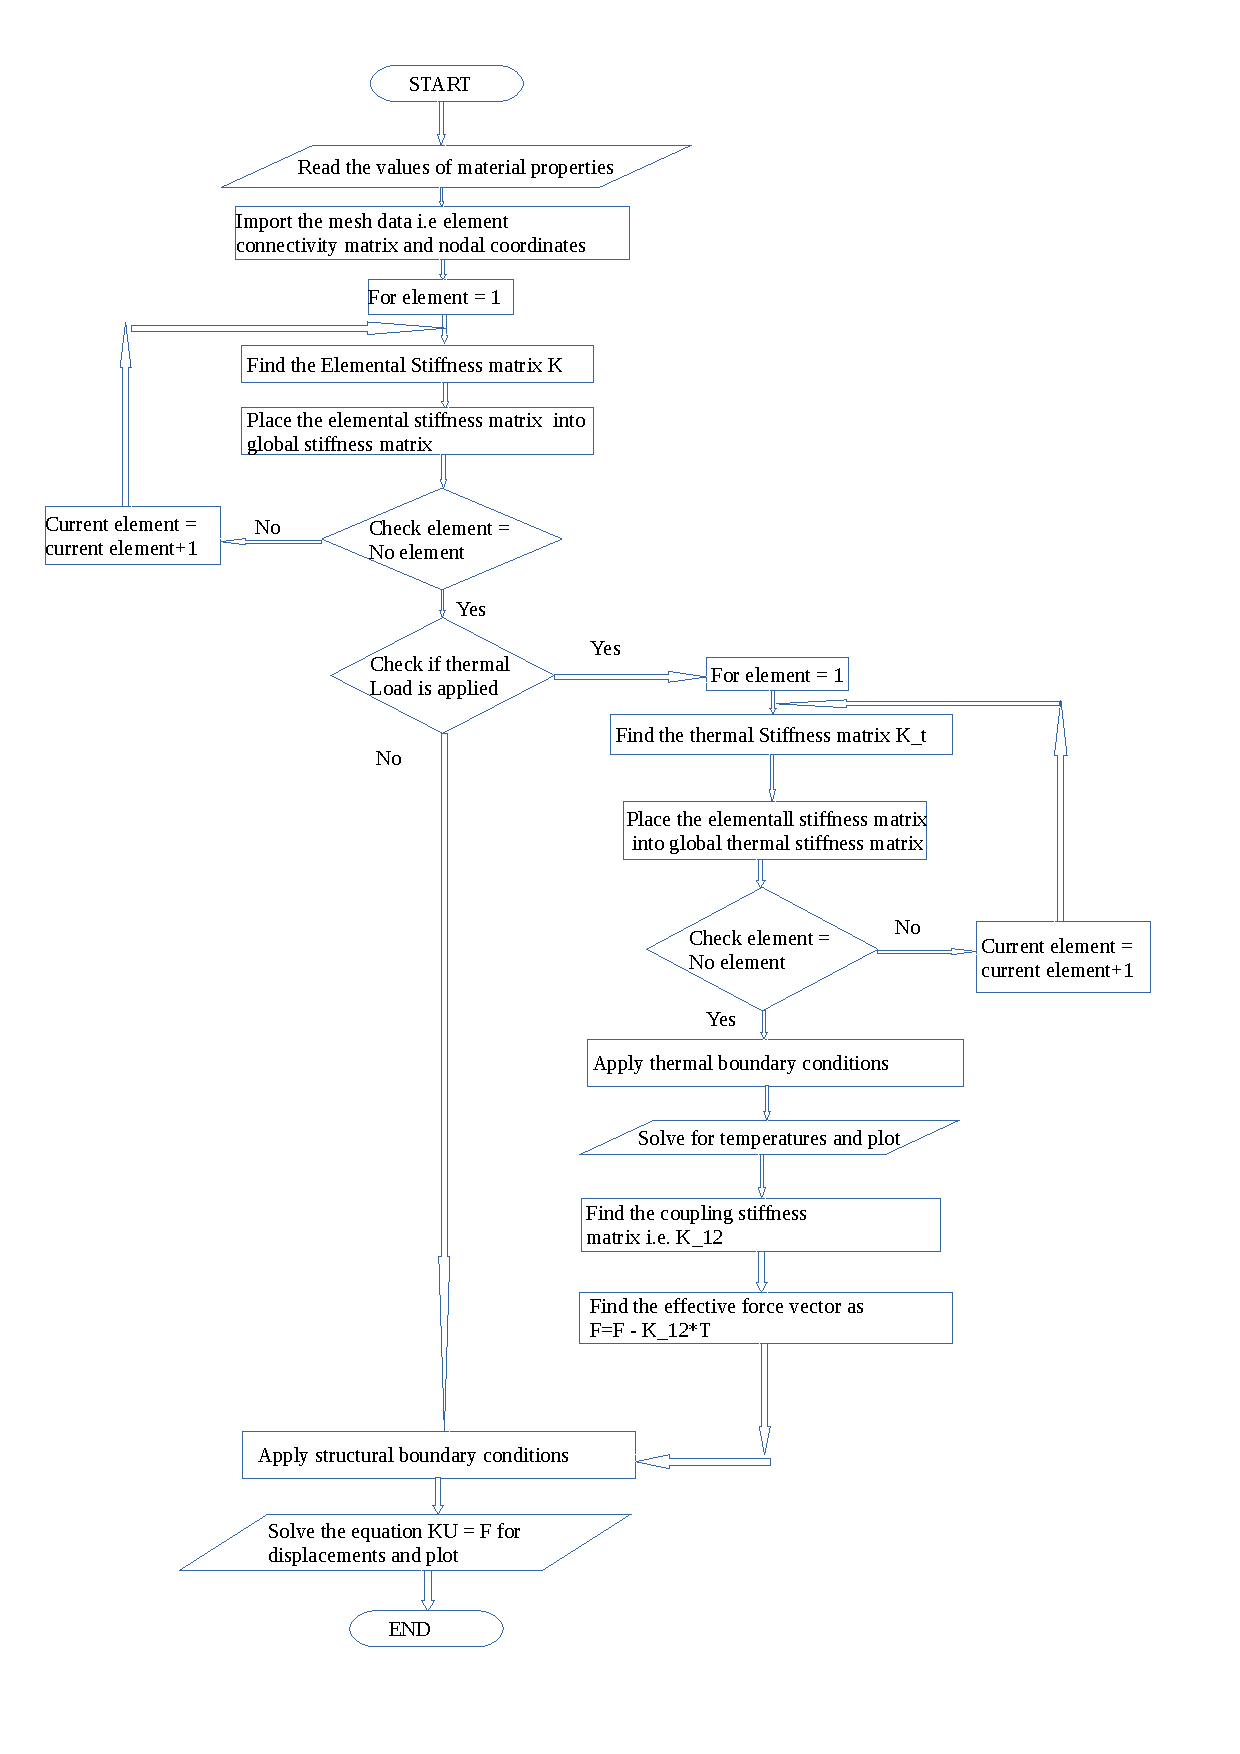
\includegraphics[width=0.48\textwidth]{flow_chart.pdf}
  \end{center}
\caption{Flowchart showing the steps of the FEM program}
\end{wrapfigure}\onslide<2->
A MATLAB program is developed to solve the 2-dimensional thermoelasticity problems.\\ \vspace{5pt}\onslide<3-> 
Quadrilateral (Q4) elements were used for meshing the body. \\ \onslide<4->\vspace{5pt}  $2\times 2$ Gauss quadrature rule is used for numerical integration.\\ \onslide<5->\vspace{5pt} 
A flow-chart showing the steps of the programming is shown in the figure.

\end{frame}
%%%%%%%%%%%%%%%%%%%%%%%%%%%%%%%%%%%%%%%%%%%%%%%%%%%%%%%%%%%%%%%%%%%%%
\begin{frame}[t,fragile]{Patch Test 1}
    \vspace{-.4cm}
    \footnotesize
 \begin{itemize}
       \onslide<2->  \item A square plate is taken and meshed with 4 elements as shown in figure below. 
        \onslide<3->  \item Minimum number of essential boundary conditions is fixed to eliminate the rigid body motions
     \onslide<4->     \item Loads are applied such that there is constant state of stress in the body
      \onslide<5->    \item Numerical integration is performed using $2\times 2$ Gauss quadrature rule.
    \end{itemize}
    \begin{figure}
    \vspace{.5cm}
\begin{subfigure}{0.45\textwidth}
    \centering \onslide<2-> 
    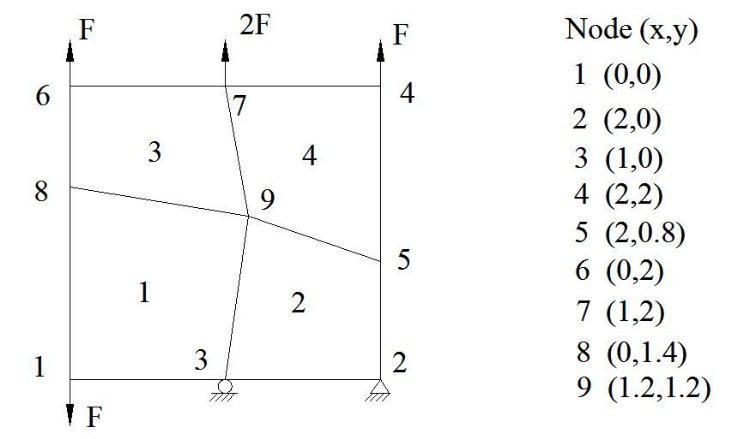
\includegraphics[scale=.25]{image1}
    \caption{\scriptsize Mesh Configuration }
\end{subfigure}
\begin{subfigure}{0.45\textwidth}
    \vspace{-.5cm}
    \centering \onslide<6-> 
\caption{\scriptsize Results of Patch Test 1} 
\scalebox{.5}{ \begin{tabular}{|c|c|c|c|c|}
\hline
& Gauss Points& $\sigma_x/2F$ & $\sigma_y/2F$ & $\tau_{xy}/2F$\\
\hline
\multirow{4}{5em}{Element 1} & 1 & $-0.222\times 10^{-15}$ & 1 & $0.1665\times 10^{-15}$\\
& 2 & $0.2498\times 10^{-15}$ & 1 & $0.1665\times 10^{-15}$\\
& 3 & $0.3058\times 10^{-15}$ & 1 & $0.222\times 10^{-15}$\\
& 4 & $0$ & 1 & $0$\\
\hline
\multirow{4}{5em}{Element 2} & 1 & $-0.222\times 10^{-15}$ & 1 & $0$\\
& 2 & $-.41633\times 10^{-15}$ & 1 & $0.111\times 10^{-15}$\\
& 3 & $0.02775\times 10^{-15}$ & 1 & $0.138\times 10^{-15}$\\
& 4 & $-0.1110\times 10^{-15}$ & 1 & $0$\\
\hline
\multirow{4}{5em}{Element 3} & 1 & $0.222\times 10^{-15}$ & 1 & $0.1665\times 10^{-15}$\\
& 2 & $0.0555\times 10^{-15}$ & 1 & $0.222\times 10^{-15}$\\
& 3 & $-0.0555\times 10^{-15}$ & 1 & $0$\\
& 4 & $0.22204\times 10^{-15}$ & 1 & $0$\\
\hline
\multirow{4}{5em}{Element 4} & 1 & $-0.222\times 10^{-15}$ & 1 & $0.1665\times 10^{-15}$\\
& 2 & $0.222\times 10^{-15}$ & 1 & $0.1665\times 10^{-15}$\\
& 3 & $0.3058\times 10^{-15}$ & 1 & $0.222\times 10^{-15}$\\
& 4 & $0.222\times 10^{-15}$ & 1 & $0$\\
\hline
\end{tabular}}
      \end{subfigure}
  \end{figure}
\end{frame}
%%%%%%%%%%%%%%%%%%%%%%%%%%%%%%%%%%%%%%%%%%%%%%%%%%%%%%%%%%%%%%%%%%%%%%%%%%%%
\begin{frame}[t,fragile]{Patch Test 2}
    \vspace{-.4cm}
    \footnotesize
 \begin{itemize}
    \onslide<2->  \item Another patch test is performed on a plate with 5 element mesh and solved and results are tabulated as shown below 
  \onslide<3->    \item The $2\times 2$ quadrature rule is used for numerical integration
    \end{itemize}
    \begin{figure}
\begin{subfigure}{0.45\textwidth}
    \centering
  \onslide<2->   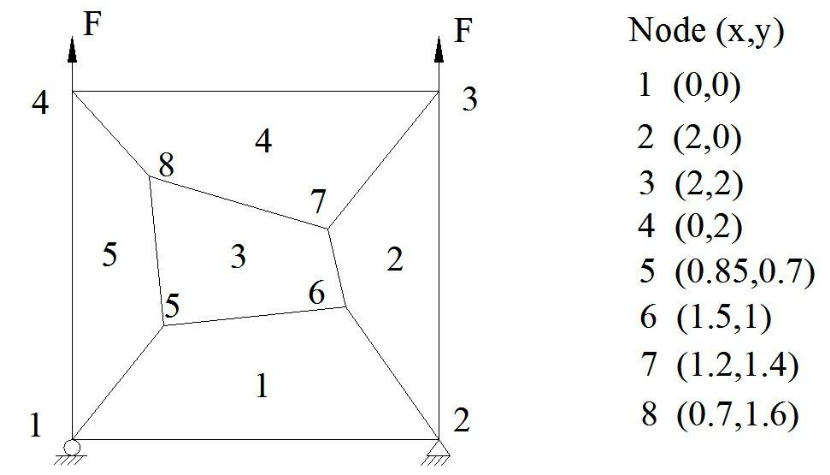
\includegraphics[scale=.2]{image2}
    \caption{\scriptsize Mesh Configuration }
\end{subfigure}
\begin{subfigure}{0.45\textwidth}
     \centering\onslide<4-> 
\caption{\scriptsize Results of Patch Test 2}
 \scalebox{.5}{\begin{tabular}{|c|c|c|c|c|}
\hline
& Gauss Point& $\sigma_x/F$ & $\sigma_y/F$ & $\tau_{xy}/F$\\
\hline
\multirow{4}{5em}{Element 1} & 1 & $0.166\times 10^{-15}$ &1& $0.1665\times 10^{-15}$\\
& 2 & $-0.033\times 10^{-15}$ &1& $0.1665\times 10^{-15}$\\
& 3 & $-0.063\times 10^{-15}$ &1& $0.222\times 10^{-15}$\\
& 4 & $0$ &1& $0$\\
\hline
\multirow{4}{5em}{Element 2} & 1 & $0.062\times 10^{-15}$ &1& $0$\\
& 2 & $-.41633\times 10^{-15}$ &1& $-0.222\times 10^{-15}$\\
& 3 & $0.02775\times 10^{-15}$ &1& $0.138\times 10^{-15}$\\
& 4 & $-0.2220\times 10^{-15}$ &1& $0$\\
\hline
\multirow{4}{5em}{Element 3} & 1 & $0.222\times 10^{-15}$ &1& $0.1665\times 10^{-15}$\\
& 2 & $0.0555\times 10^{-15}$ &1& $0.222\times 10^{-15}$\\
& 3 & $-0.0555\times 10^{-15}$ &1& $0$\\
& 4 & $0.22204\times 10^{-15}$ &1& $0$\\
\hline
\multirow{4}{5em}{Element 4} & 1 & $-0.222\times 10^{-15}$ &1& $0.1665\times 10^{-15}$\\
& 2 & $0.222\times 10^{-15}$ &1& $0.1665\times 10^{-15}$\\
& 3 & $-0.063\times 10^{-15}$ &1& $0.222\times 10^{-15}$\\
& 4 & $0.222\times 10^{-15}$ &1& $0$\\
\hline
\multirow{4}{5em}{Element 5} & 1 & $-0.422\times 10^{-15}$ &1& $0.1665\times 10^{-15}$\\
& 2 & $0.222\times 10^{-15}$ &1& $0.1665\times 10^{-15}$\\
& 3 & $-0.063\times 10^{-15}$ &1& $0.222\times 10^{-15}$\\
& 4 & $0.222\times 10^{-15}$ &1& $0$\\
\hline
\end{tabular}}
     \end{subfigure}
  \end{figure}
\end{frame}
%%%%%%%%%%%%%%%%%%%%%%%%%%%%%%%%%%%%%%%%%%%%%%%%%%%%%%%%%%%%%%%%%%%%%%%%%%%%
\begin{frame}[t,fragile]{Patch Test 3 : Thermal code }
    \vspace{-.4cm}
 \begin{itemize}
    \onslide<2->  \item Another patch was performed to validate the thermal code.
   \onslide<3->   \item Same problem as patch test was taken 
  \onslide<4->    \item Temperature loads are applied to get the constant heat flux throughout the body
    \end{itemize}
    \begin{figure}
    \vspace{.5cm}
    \hspace{-.5cm}
\begin{subfigure}{0.3\textwidth}
     \centering
   \onslide<2->  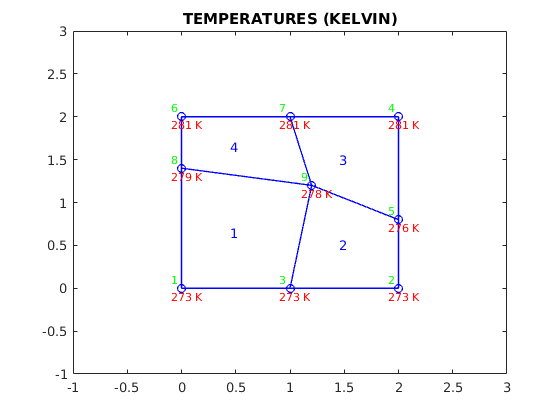
\includegraphics[scale=.2]{solution.jpg}
    \caption{\tiny Temperature distribution}
\end{subfigure}
\begin{subfigure}{0.6\textwidth}
    \vspace{-1cm}
    \centering
    \onslide<5-> \caption{\scriptsize Results of Patch test 3}
 \scalebox{.55}{\begin{tabular}{|C{3cm}|C{3cm}|C{3cm}|C{3cm}|}
        \hline
        Nodes&Temperatures&$Q_y(W)$&$Q_x(W)$\\
        \hline
        1&273&200&$0.125\times 10^{-10}$\\
        \hline
        2&273&200&$0.155\times 10^{-10}$\\
        \hline
        3&273&200&$0.222\times 10^{-10}$\\
        \hline
        4&281&200&0\\
        \hline
        5&276&200&$0$\\
        \hline
        6&281&200&$0$\\
        \hline
        7&281&200&$0.111\times 10^{-10}$\\
        \hline
        8&279&200&$0.138\times 10^{-10}$\\
        \hline
        9&278&200&$0$\\
        \hline
    \end{tabular}}
     \end{subfigure}
  \end{figure}
\end{frame}
%%%%%%%%%%%%%%%%%%%%%%%%%%%%%%%%%%%%%%%%%%%%%%%%%%%%%%%%%%%%%%%%%%%%%%%%%
\begin{frame}[t,fragile]{Patch Test 4: Thermo-elastic code}
    \vspace{-.5cm}
    \footnotesize\onslide<2-> 
\begin{figure}[H]
    \centering
    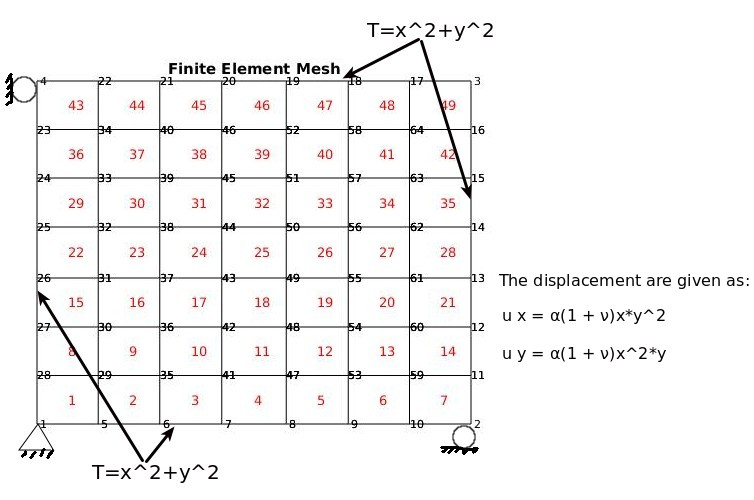
\includegraphics[scale=.2]{elements_7^2_1.jpg}
\end{figure}
    \vspace{-.5cm}
\begin{itemize}
  \onslide<2->   \item A square plate of dimension $2\times 2$ is taken and meshed as shown
 \onslide<3->    \item Temperature distribution of $T=x^2+y^2$ is applied on 4 boundaries of plate
 \onslide<4->    \item a heat source $q=\frac{\partial^2 T}{\partial x^2}+\frac{\partial^2 T}{\partial y^2}=4$ is applied throughout the body 
    \item Mesh is refined and to get the more accurate results 
\end{itemize}
\end{frame}
%%%%%%%%%%%%%%%%%%%%%%%%%%%%%%%%%%%%%%%%%%%%%%%%%%%%%%%%%%%%%%%%%%%%%%% 
\begin{frame}[t,fragile]{Mesh Refinements}
    \onslide<2->\begin{figure}
    \centering  
\begin{tikzpicture}[      
        every node/.style={scale=.6,anchor=south west,inner sep=0pt},
        x=1mm, y=1mm,scale=.6
      ] 
       \node (fig2) at (-25,-35)
      {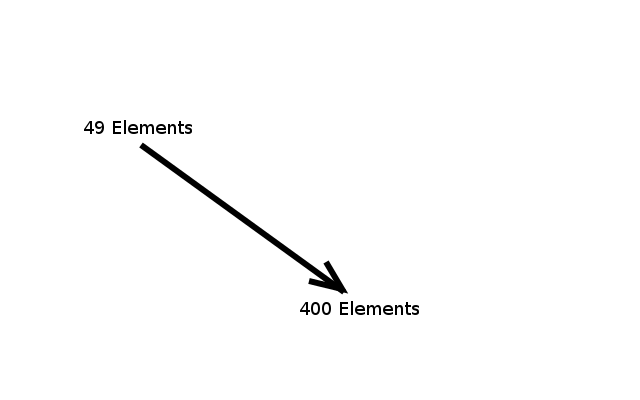
\includegraphics[scale=0.35]{arrow}};  
       \node (fig1) at (0,0)
      {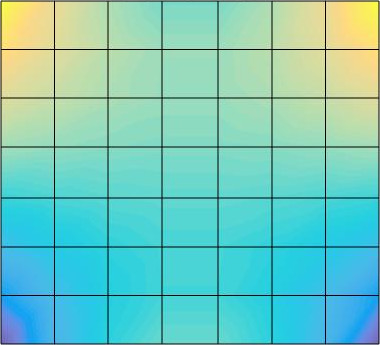
\includegraphics[scale=0.3]{uy_7^2}};
      \node (fig2) at (10,-10)
    {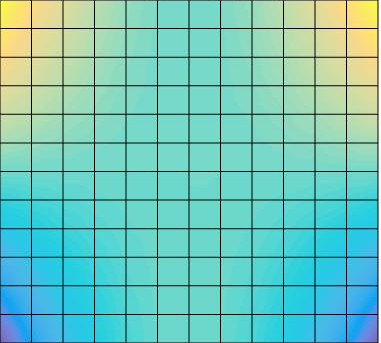
\includegraphics[scale=0.3]{uy_12^2}};
       \node (fig2) at (20,-20)
       {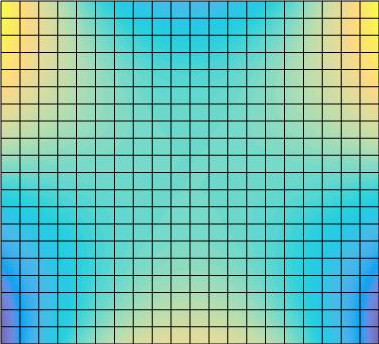
\includegraphics[scale=0.3]{uy_20^2}};  
    \end{tikzpicture}
\end{figure}\onslide<3->
 \vspace{-1cm}\begin{figure}
   \centering 
  \caption{\scriptsize Errors obtained after mesh refinements }
    \vspace{-16pt}
 \scalebox{.6}{\begin{tabular}{|c|c|c|c|c|c|}
        \hline
       Number of Elements & Error in  $u_x$ & Error in  $u_y$ & Error in  $\sigma_x$ & Error in  $\sigma_y$ & Error in  $\tau_{xy}$\\
        \hline
       $7\times 7$ & $5.783469\times 10^{-10}$ & $5.783469\times 10^{-10}$ & $6.668255\times 10^{2}$ & $6.668255\times 10^{2}$ & $3.615391\times 10^{2}$\\
        \hline
         $12\times 12$ & $1.764697\times 10^{-11}$ & $1.764697\times 10^{-11}$ & $1.000597121$ & $1.000597121$ & $0.031722$\\
        \hline
        $20\times 20$ & $1.265804\times 10^{-12}$ & $1.265804\times 10^{-12}$ & $0.994299467$ & $0.994299467$ & $0.005781$\\
        \hline
    \end{tabular}}
\end{figure}
\end{frame}
%%%%%%%%%%%%%%%%%%%%%%%%%%%%%%%%%%%%%%%%%%%%%%%%%%%%%%%%%%%%%%%%%%%%%%%%%
\begin{frame}[t,fragile]{Plate with edge crack}
    \vspace{-.4cm}
    %%%%%%%%%%%%%
   \begin{figure}[H]
    \centering
        \begin{subfigure}{.3\textwidth}
       \onslide<2->      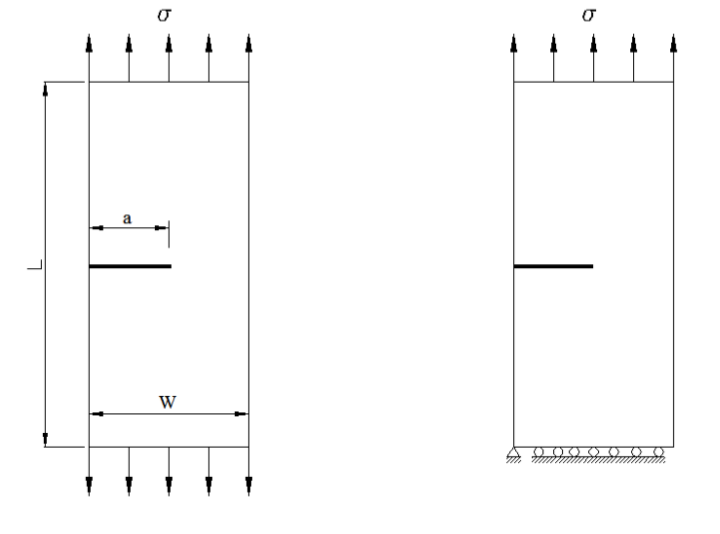
\includegraphics[scale=.15]{mai.png}
            \caption{\scriptsize Plate with edge crack}
    \end{subfigure}
    \hspace{5pt}
        \begin{subfigure}{.3\textwidth}
      \onslide<4->       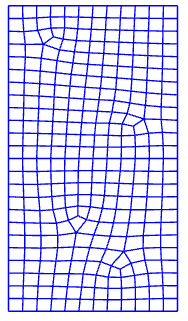
\includegraphics[scale=.22]{untitled1.png}
            \caption{\scriptsize Before loading}
    \end{subfigure}
        \begin{subfigure}{.3\textwidth}
       \onslide<4->      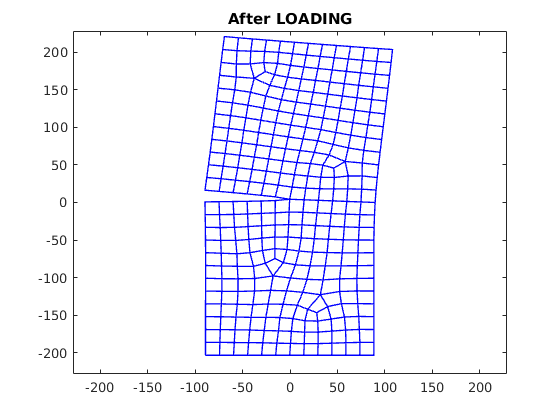
\includegraphics[scale=.22]{untitled2.png}
            \caption{\scriptsize After loading}
    \end{subfigure}
        \vspace{-10pt}
    \end{figure}
    \vspace{20pt}
    \footnotesize
    \begin{itemize}
    \onslide<2->     \item A plate with edge crack is meshed in ANSYS and imported to MATLAB
     \onslide<3->    \item Boundary conditions are applied and stresses ahead of cracktip is plotted
     \onslide<4->    \item The results obtained by MATLAB code is compared with the ANSYS solution
    \end{itemize}
\end{frame}
    %%%%%%%%%%%%%%%%%%%%%%%%%%%%%%%%%%%%%%%%%%%%%%%%%%%%%%%%%%%%%%%%%%%%%
\begin{frame}[t,fragile]{Stresses Ahead of Crack-tip: Comparison with ANSYS}
    \vspace{-10pt}
    \begin{figure}
        \centering
        \hspace{22pt}
        \begin{subfigure}{.3\textwidth}
      \onslide<2->  {     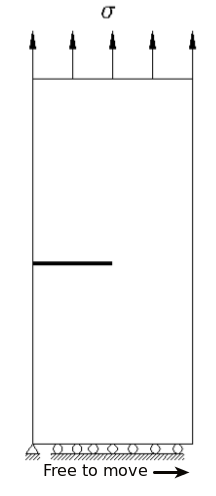
\includegraphics[scale=.20]{3.png}}
    \end{subfigure}
    \begin{subfigure}{.3\textwidth}
      { \vspace{10pt}
   \onslide<3->  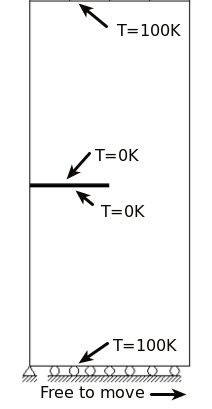
\includegraphics[scale=.20]{4.png}}
    \end{subfigure}
    \begin{subfigure}{.3\textwidth}
    {    \vspace{-10pt}
 \onslide<4-> 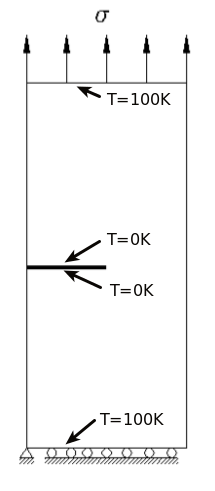
\includegraphics[scale=.20]{5.png}}
        \vspace{-10pt}
    \end{subfigure}
    \end{figure}
    %%%%%%%%%%%%%%%
    \vspace{-10pt}
    \begin{figure}
    \begin{subfigure}{.3\textwidth}
     \onslide<2->  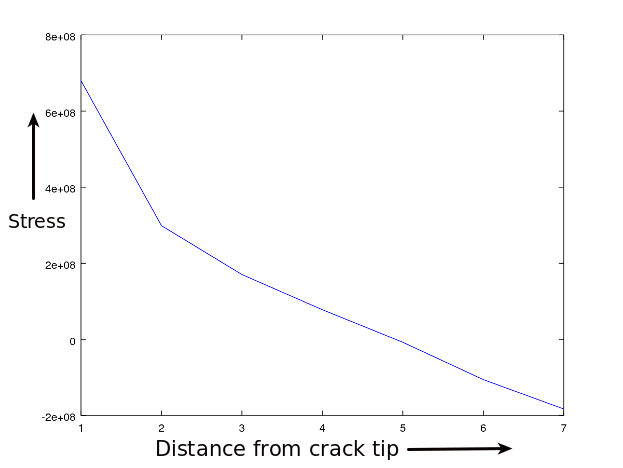
\includegraphics[scale=.2]{onlystress}
\caption{\tiny $\sigma_y$ ahead of the crack tip}
    \label{stress}
\end{subfigure}
\hspace{1pt}
    \begin{subfigure}{.3\textwidth}
    \centering
    \onslide<3-> 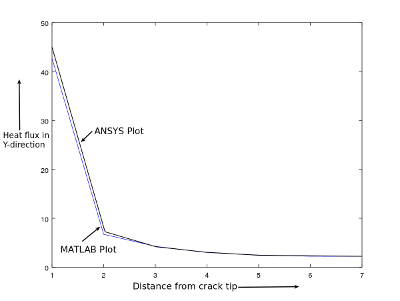
\includegraphics[scale=.25]{onlytempqy}
\caption{\tiny Heat flux ahead of crack tip}
    \label{fig:heat}
\end{subfigure}
\hspace{1pt}
    \begin{subfigure}{.3\textwidth}
    \onslide<4->     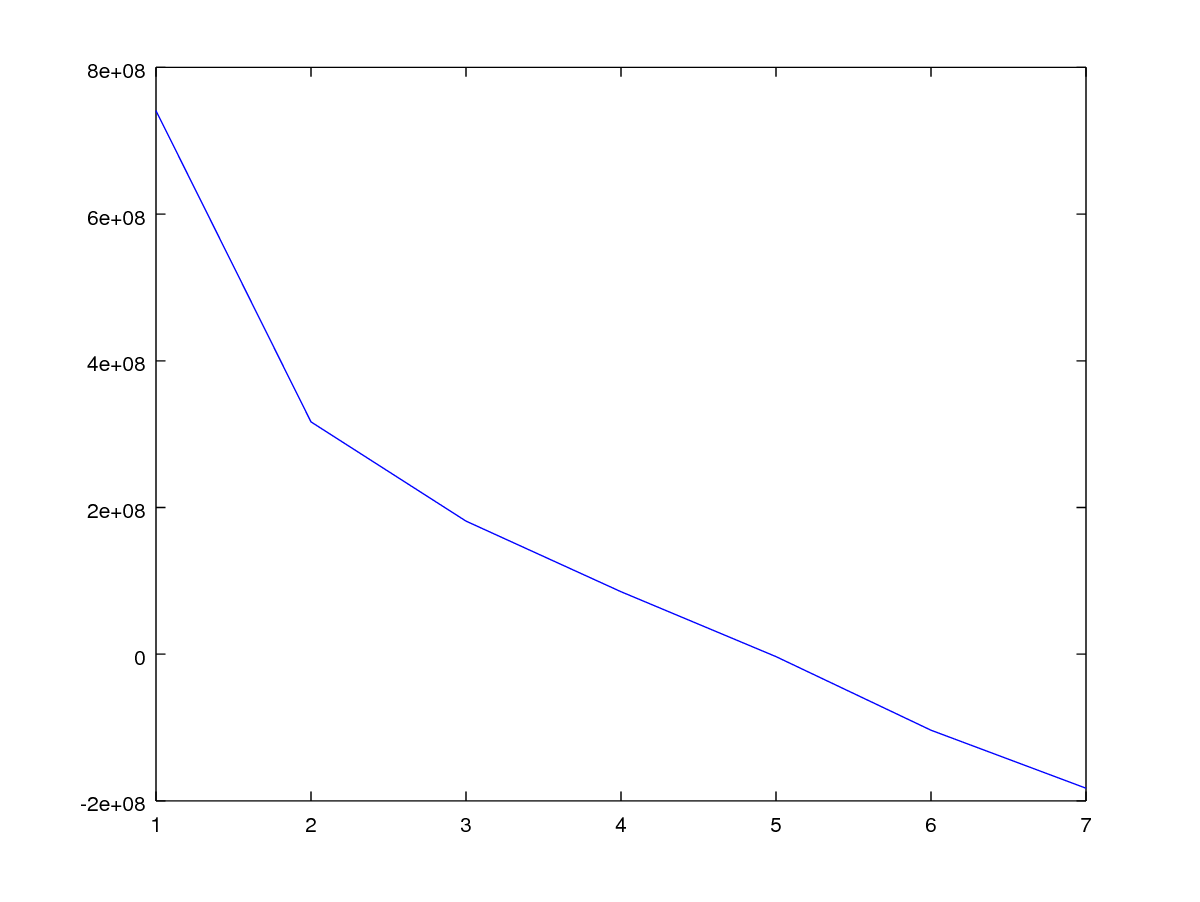
\includegraphics[scale=.2]{only_bothstress}
   \caption{\tiny $\sigma_y$ ahead of the crack tip}
    \label{heat1}
\end{subfigure}
\end{figure}
\end{frame}
%%%%%%%%%%%%%%%%%%%%%%%%%%%%%%%%%%%%%%%%%%%%%%%%%%%%%%%%%%%%%%%5
\begin{frame}[t,fragile]{Comparison of FEM and X-FEM methods}
    \vspace{-.7cm}
    \hspace{15pt}
     \onslide<2->  \begin{figure}[H]
    \begin{subfigure}{0.45\textwidth}
    \centering
    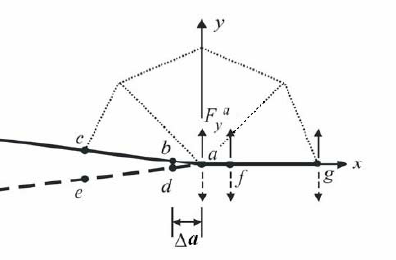
\includegraphics[scale=.2]{crackclosure.png}
    \caption{\tiny Crack closure technique}
\end{subfigure}
        \hspace{15pt}
       \begin{subfigure}{0.45\textwidth}
    \centering
      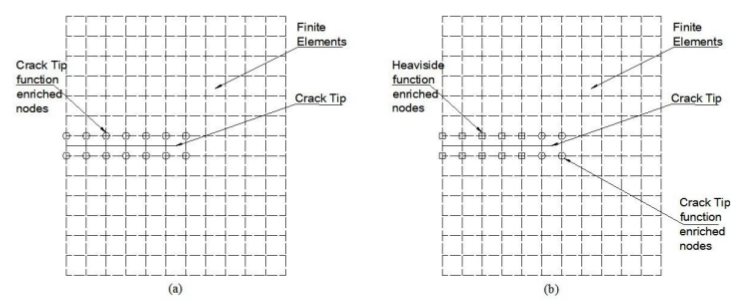
\includegraphics[scale=.15]{k.png}
    \caption{\tiny X-FEM enrichment of nodes}
\end{subfigure}
\end{figure}
\vspace{-12pt}
    \tiny \onslide<3->  
\begin{align*}
    \onslide<3->  \text{Crack closure integral:}\ \ \ \ \ \ \ G_I=\frac{W}{B\Delta a}=\frac{F_{y}^au_{y}^b}{2B \Delta a}\ \ \ Thus, \ \ \ \
    K_I&=\sqrt{\frac{G_I}{E}}=5.24586910\times 10^9\ \ Pa\sqrt{m}\\ 
   \text{Analytical:}\ \ \ \ \ \ \ K_I=C*\sigma\sqrt{\pi a}=4.726065 \times 10^9\ \ Pa\sqrt{m}\\
\end{align*}
\vspace{-28pt}
\bgroup
\def\arraystretch{2}\onslide<4->  
\begin{table}[H]
    \centering
    \begin{tabular}{|C{3cm}|C{6cm}|}
\hline 
Method used& $\% \ Error= \{K_{theoretical}-K_{numerical}/K_{theoretical}\}\times 100$\\
\hline
 Finite Element Method & 11.1\%\\
\hline
 Extended Finite Element Method& 4\%\\
\hline
\end{tabular}
\label{table1}
\end{table}
\egroup
\end{frame} 
%%%%%%%%%%%%%%%%%%%%%%%%%%%%%%%%%%%%%%%%%%%%%%%%%%%%%%%%%%%%%%%
\begin{frame}[t,fragile]{Conclusions}
    \vspace{-.2cm}
    \footnotesize
\begin{itemize}
  \onslide<2->     \item A semi-coupled thermoelastic problem is formulated, FEM program is developed in MATLAB and validated by performing different patch tests.
    \onslide<3->   \item It is shown that when solving fracture problems with traditional FEM program, solutions are not accurate around the crack tip
   \onslide<4->    \item Same problem is solved in an X-FEM program developed by parnaik to show that the solution improves drastically when using X-FEM
    \onslide<5->   \item The Extended Finite Element enrichments will be applied to both displacement and temperature fields of thermoelasticity program in stage 2 of the project  
   \onslide<6->    \item Q8 elements will be applied in our program to solve curved boundary problems. 
   \onslide<7->    \item As the hydrogen diffusion in cracked bodies are governed by the Poisson's equation similar to the thermoelastic problems, we will modify the X-FEM program to solve problems of hydrogen-diffusion 
    \end{itemize}
\end{frame}
%%%%%%%%%%%%%%%%%%%%%%%%%%%%%%%%%%%%%%%%%%%%%%%%%%%%%%%%%%%%%%%%%
\begin{frame}[t,fragile]{References}
    \tiny
\begin{thebibliography}{10}
      \bibitem{prashant} Kumar, P., \& Prashant, K. (2009). Elements of fracture mechanics. Tata McGraw-Hill Education.
      \bibitem{filery} Fillery, B. P., Hu, X., \& Fisher, G. (2006). Thermo-elastic fracture of edge cracked plate under surface ‘shock’loading. In \emph{Fracture of Nano and Engineering Materials and Structures} (pp. 385-386). Springer Netherlands.
      \bibitem{tian} Tian, X., Shen, Y., Chen, C., \& He, T. (2006). A direct finite element method study of generalized thermoelastic problems. International Journal of Solids and Structures, 43(7), 2050-2063.
      \bibitem{sih} Sih, G. C. (1962). On the singular character of thermal stresses near a crack tip. Journal of Applied Mechanics, 29(3), 587-589.
      \bibitem{helen} Hellen, T. K., \& Cesari, F. (1979). On the solution of the centre cracked plate with a quadratic thermal gradient. \emph{Engineering Fracture Mechanics}, 12(4), 469-478.
      \bibitem{belytsko} Belytschko, T., \& Black, T. (1999). Elastic crack growth in finite elements with minimal remeshing. \emph{International journal for numerical methods in engineering}, 45(5), 601-620.
      \bibitem{koustubh} Koustubh Parnaik. (2013). Implementation of Extended Finite Element Method (X-FEM) for static fracture problems. \emph{Department of Mechanical Engineering, IIT Bombay}.
     \bibitem{duflot} Duflot, M. (2008). The extended finite element method in thermoelastic fracture mechanics. \emph{International Journal for Numerical Methods in Engineering}, 74(5), 827-847.
     \bibitem{budyn} Budyn, E., Zi, G., Moës, N., \& Belytschko, T. (2004). A method for multiple crack growth in brittle materials without remeshing. \emph{International journal for numerical methods in engineering}, 61(10), 1741-1770.
\end{thebibliography}
\end{frame}
\begin{frame}[t,fragile]{\ldots References}
    \tiny
\begin{thebibliography}{10}
     \bibitem{stazi} Stazi, F. L., Budyn, E., Chessa, J., \& Belytschko, T. (2003). An extended finite element method with higher-order elements for curved cracks. \emph{Computational Mechanics}, 31(1-2), 38-48.
     \bibitem{khoei} Khoei, A. R., \& Nikbakht, M. (2007). An enriched finite element algorithm for numerical computation of contact friction problems. \emph{International Journal of Mechanical Sciences}, 49(2), 183-199.
     \bibitem{liang} Liang, J., Huang, R., Prevost, J. H., \& Suo, Z. (2003). Evolving crack patterns in thin films with the extended finite element method. \emph{International Journal of Solids and Structures}, 40(10), 2343-2354.
     \bibitem{yangzian} Xu, Y., \& Yuan, H. (2009). On damage accumulations in the cyclic cohesive zone model for X-FEM analysis of mixed-mode fatigue crack growth.\emph{Computational Materials Science}, 46(3), 579-585.
     \bibitem{atkinson} Atkinson, K. E. (1997). \emph{The numerical solution of integral equations of the second kind} (Vol. 4). Cambridge university press.
    \bibitem{sad} Sad, M. H. (2004). Elasticity: Theory. \emph{Applications and Numerics}. 
    \bibitem{reddy} Reddy, J. N. (1989). An introduction to the finite element method.
    \bibitem{belytsko2} Fries, T. P., \& Belytschko, T. (2010). The extended/generalized finite element method: an overview of the method and its applications. \emph{International Journal for Numerical Methods in Engineering}, 84(3), 253-304.
    \bibitem{karihaloo} Liu, X. Y., Xiao, Q. Z., \& Karihaloo, B. L. (2004). X-FEM for direct evaluation of mixed mode SIFs in homogeneous and bi‐materials. \emph{International Journal for Numerical Methods in Engineering}, 59(8), 1103-1118.
\end{thebibliography}
\end{frame}
\end{document}
